\documentclass[11pt,a4paper]{article}
\usepackage[T1]{fontenc}
\usepackage[utf8]{inputenc}
\usepackage{lmodern}
\usepackage[margin=2.3cm]{geometry}
\usepackage{booktabs,tabularx,array,graphicx,enumitem,microtype,float}
\usepackage[font=small,justification=raggedright,singlelinecheck=false]{caption}
\usepackage[hidelinks]{hyperref}
\setlength{\parskip}{0.45em}
\setlength{\parindent}{0pt}
\setlist{itemsep=0.15em,topsep=0.3em}
\newcolumntype{L}{>{\raggedright\arraybackslash}X}
\renewcommand{\arraystretch}{1.2}

\title{\textbf{Synthetic customers: do LLM twins answer like real respondents?}\\[0.4em]
\large Individual AI Project, 20595 Business Analytics}
\author{Benedetta Gatto (3341868)\\Prof.\ Abhinav Pandey, Bocconi University}
\date{November 2026}

\begin{document}
\maketitle

\begin{abstract}
\noindent Synthetic customers built from real respondents' demographics do not reproduce how real customers respond to price. They answer in a strict step pattern, are about twice as price sensitive and always take a free product. The pattern holds for two models from different companies, but the twin of the same person changes a lot between models. Income gaps are too small in the real data to test whether the twins reproduce them. Repository: \texttt{github.com/benedettagattoo/synthetic-customers-individual-ai-project}.
\end{abstract}

%=====================================================
\section{Question and theory}

\textbf{Question.} Do LLM-generated synthetic customers, given only the demographics of real respondents, reproduce the differences between income groups in purchase intention seen in the real data? The question is about groups, not individuals.

\textbf{Theory.} Argyle et al.\ (2023) find that models given people's backgrounds reproduce how groups answer, so the direction of income gaps should match. Bisbee et al.\ (2024) and Wang et al.\ (2025) find too little variation and flattened within-group differences, so the size of the gaps and the overall purchase rate should not match.

\begin{table}[H]
\centering\small
\begin{tabularx}{\linewidth}{lLL}
\toprule
\textbf{Hypothesis} & \textbf{Statement} & \textbf{Proved wrong if (fixed in plan.md before any synthetic answer)}\\
\midrule
H1 direction & Sign of the high- minus low-income gap is the same for synthetic and real & Opposite sign for half or more of the products, or correlation of gaps $\le 0$\\
H2 size & Synthetic gaps differ in size from real gaps & Synthetic gaps fall inside the real 95\% CI\\
H3 level & Overall synthetic purchase rate differs from the real one & Synthetic rate inside the real 95\% CI\\
H4 price sensitivity & Synthetic slope of Yes share on relative price matches the real slope & Synthetic slope outside the real CI, or of opposite sign, for half or more of the products\\
H5 income gradient & Synthetic high- minus low-income slope gap has the real sign & Sign disagrees for half or more of the testable products\\
\bottomrule
\end{tabularx}
\caption{Hypotheses and falsification rules. A product whose real gap CI covers 0 cannot test direction (H1, H5) and is reported separately.}
\end{table}

%=====================================================
\section{Data and design}

The comparison uses 200 real respondents, 40 per income bracket, and one synthetic twin for each, on 10 products at 11 prices.

\begin{itemize}
\item \textbf{Data.} Twin-2K-500 (LLM-Digital-Twin/Twin-2K-500, CC BY 4.0): 2,058 US respondents. Income is QID21 (5 brackets, waves 1--3). The outcome is Yes/No purchase intention in the wave-4 pricing study, where each respondent saw each of 40 products at one random price.
\item \textbf{Exclusions.} 79 respondents have a malformed price string (41--44 item:price pairs instead of 40) and are excluded from everything that uses prices: 1,979 valid.
\item \textbf{Products.} QID9\_k is the $k$-th product displayed, not a fixed product (display order is randomised per respondent). Products are therefore tracked by item number; 10 items are chosen by a fixed rule (every 4th display position of respondent 1): 25, 27, 31, 9, 36, 26, 15, 23, 38, 10.
\item \textbf{Prices.} Each item has an 11-point ladder from \$0 (``product is free'') to about twice the base price. Relative price = price / ladder maximum.
\item \textbf{Sample.} 200 respondents stratified by income (40 per bracket, seed 20261111). Respondent IDs were replaced by C001--C200 before anything was sent to a model.
\item \textbf{Synthetic step (Gabor-Granger).} Each twin receives its real respondent's demographics and, in one call per product, answers Yes/No at all 11 prices, shown in random order (seed 20261112): 2,000 calls, 22,000 answers.
\item \textbf{Model.} \texttt{gemini-3.5-flash-lite} (Google AI Studio, version 3.5-flash-lite-07-2026, temperature 1), fixed in plan.md before any answer. Robustness model: \texttt{gpt-oss:20b} via Ollama 0.40.16 on the Bocconi HPC (Section~\ref{sec:rob}).
\item \textbf{Estimation.} Linear probability models of Yes on relative price plus a free-price indicator, with item fixed effects; 95\% CIs by bootstrap over respondents or twins (B = 2,000, seed 20261112); clustered standard errors in the joint models.
\end{itemize}

Because each real respondent saw one price per product while each twin saw the whole ladder, the twin-level comparison (H1--H3) uses the synthetic answer at the real respondent's own price; the curve comparison (H4--H5) uses all 11 prices.

%=====================================================
\section{Results}

The synthetic twins buy slightly more often than real people, are about twice as price sensitive, and always take a free product; the income questions cannot be answered because real income gaps are near zero.

\begin{table}[H]
\centering\small
\begin{tabularx}{\linewidth}{lLL}
\toprule
\textbf{Hypothesis} & \textbf{Result (Gemini)} & \textbf{Verdict}\\
\midrule
H1 direction & Only 1 of 10 products has a real income gap whose CI excludes 0; the sign agrees on it; correlation of gaps over all 10 = 0.28 & Not rejected, but essentially untested\\
H2 size & Synthetic gap inside the real 95\% CI for 7 of 10 products & ``Rejected'' by the rule, but real CIs are about $\pm 0.20$ wide (40 twins per bracket): low power, not evidence that sizes match\\
H3 level & Synthetic Yes rate at the real price 0.516 vs real 0.475 [0.449, 0.502] & Not rejected: rates differ\\
H4 price sensitivity & All 10 synthetic slopes outside the real CI; pooled slope $-1.398$ [$-1.403$, $-1.392$] vs real $-0.686$ [$-0.710$, $-0.662$] & Rejected (10 of 10 products)\\
H5 income gradient & Real high- minus low-income slope gap $+0.014$ [$-0.060$, $+0.085$]; 0 testable products & Cannot test\\
\bottomrule
\end{tabularx}
\caption{Verdicts. Files: \texttt{results/compare1\_hypotheses.csv}, \texttt{compare1\_gaps.csv}, \texttt{compare2\_hypotheses.csv}, \texttt{compare2\_h4\_h5.csv}.}
\end{table}

\begin{figure}[H]
\centering
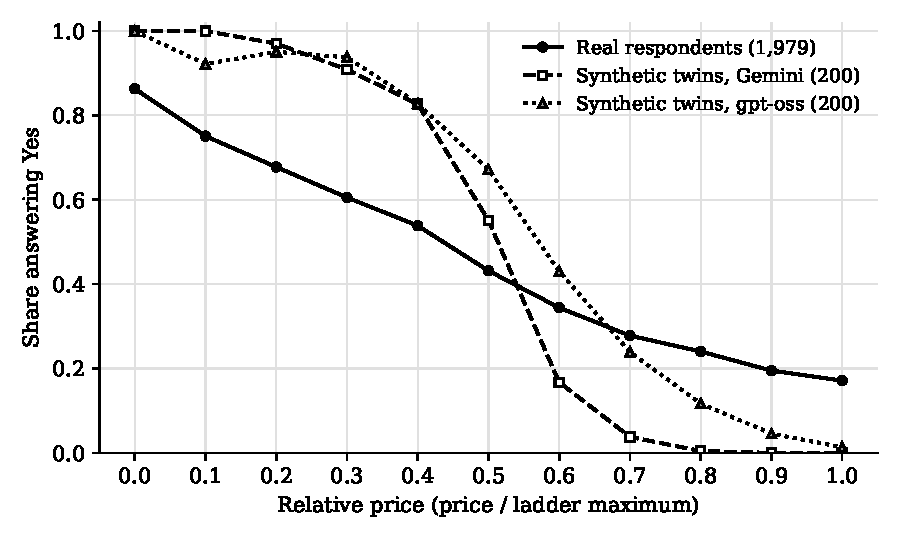
\includegraphics[width=0.82\linewidth]{curve_bw.pdf}
\caption{Pooled demand curves over the 10 products. Real demand falls gradually from 0.86 at \$0 to 0.17 at the top of the ladder; synthetic demand stays near 1 up to the middle of the ladder and then collapses. Each individual twin answers with a single step; the pooled synthetic curves are smoothed only because twins place the step at slightly different prices. Source: \texttt{results/real\_demand\_curves.csv}, \texttt{compare2\_curves\_synthetic.csv}, \texttt{robust\_compare2\_curves\_synthetic.csv}.}
\end{figure}

\textbf{Shape of demand.} Every one of the 2,000 Gemini ladders is a single step: Yes up to a threshold, No above it, never back. 77\% of thresholds sit at 5--6 Yes answers, around the base price.

\textbf{Free products.} Synthetic twins said Yes to every free product (2,000 of 2,000); real respondents 86.3\% (1,495 of 1,732). I recomputed this number by hand.

\textbf{Reading the slopes.} Synthetic LPM slopes below $-1$ are an artefact of fitting a straight line to a step: the direction (far more price sensitive) is clear, but the magnitude is not a meaningful elasticity. The curves describe the shape better than the slope.

\textbf{Twin by twin.} At the real respondent's own price, the twin gives the same answer in 72.75\% of the 2,000 pairs (exploratory, not part of any hypothesis).

%=====================================================
\section{Robustness: a second model}\label{sec:rob}

A model from a different company, \texttt{gpt-oss:20b}, gives the same H3 and H4 verdicts and the same step pattern, so the main conclusion is robust to the model; the individual twins are not.

The same 2,000 prompts, price orders and validation were run in one Slurm job on the Bocconi HPC (A100 MIG slice, 8~h~56~min). The reading rule was fixed in plan.md before any gpt-oss answer was analysed: the result is robust if the H3 and H4 verdicts match Gemini and at least 90\% of gpt-oss ladders are single-threshold.

\begin{table}[H]
\centering\small
\begin{tabular}{lccc}
\toprule
\textbf{Measure} & \textbf{Real} & \textbf{Gemini} & \textbf{gpt-oss:20b}\\
\midrule
Yes share at \$0 & 0.863 & 1.000 & 0.9995\\
Single-threshold ladders & not defined & 1.000 & 0.906\\
Pooled slope on relative price & $-0.686$ & $-1.398$ & $-1.250$\\
Yes rate at the real price (H3) & 0.475 & 0.516 & 0.572\\
H4 verdict & & Rejected 10/10 & Rejected 10/10\\
\bottomrule
\end{tabular}
\caption{Robustness. Sources (results/): robustness\_summary.csv, robust\_compare1\_hypotheses.csv and robust\_compare2\_hypotheses.csv, made by src/10\_robustness\_summary.py.}
\end{table}

Two caveats:
\begin{itemize}
\item \textbf{The 90\% condition is met narrowly (0.906).} Of the 189 other gpt-oss ladders, 156 switch three times (Yes, No, Yes, No as price rises), which makes no economic sense.
\item \textbf{Agreement is aggregate only.} The two models give the same answer in 87.1\% of the 22,000 cells, but where both answer with a single step they put the threshold at the same price for only 27.7\% of ladders (502 of 1,811); gpt-oss buys on average 0.7 ladder steps higher. The same person's twin changes with the model.
\end{itemize}

\textbf{Checks.} Sixteen gpt-oss keys had been excluded because prices were written without the dollar sign; they were recovered by an offline re-validation rule fixed before any answer was analysed. Without these 16 keys, and separately for the two output formats (70 vs 1,930 keys), the headline numbers barely move (single-threshold 0.905 / 0.914 / 0.905). H1, H2 and H5 are reported side by side without a robustness claim (low power).

%=====================================================
\section{Verification}

Every headline number was recomputed outside the script that produced it; the headline number was recomputed by me by hand, without any agent. Full log: mistakes.md.

\begin{table}[H]
\centering\footnotesize
\begin{tabularx}{\linewidth}{>{\raggedright\arraybackslash}p{2.4cm}L>{\raggedright\arraybackslash}p{2.7cm}>{\raggedright\arraybackslash}p{1.9cm}L}
\toprule
\textbf{What} & \textbf{How} & \textbf{Against what} & \textbf{Who} & \textbf{Outcome}\\
\midrule
Headline: Yes share when free & Filtered the CSVs in Numbers & synthetic\_\allowbreak{}answers.csv, real\_\allowbreak{}items\_\allowbreak{}long.csv & Me, no agent & Passed: 2,000/2,000 and 1,495/1,732\\
First data report: three agent claims & Opened the raw files & data/raw & Me & Checks a and b passed; check c found a column range described wrongly (12 IDs vs 10 columns), so a rule was added to AGENTS.md\\
QID9\_\allowbreak{}k = product? & Compared the catalog with randDollarsString & 40/40 positions of respondent 1 & Me, with Claude & Assumption wrong: QID9\_\allowbreak{}k is a display position; plan corrected\\
Sample is reproducible & Re-ran src/01\_\allowbreak{}prepare.py & Previous output & Agent, checked by me & 0 mismatches\\
Real demand curves and slopes & Independent recomputation of item 38 (55 cells) and of slopes for items 31, 27 and pooled & results/real\_\allowbreak{}*.csv & With Claude & 0 differences\\
Agent run vs workflow run & Row-by-row comparison & results/agent\_\allowbreak{}run vs results/ & With Claude & Identical, because the agent copied the choices from plan.md: not independent (mistakes.md 29)\\
Comparison scripts 07 and 08 & Internal consistency checks and independent recomputation of the 2,000 pairs & Script output & Agent and Claude & Two bugs caught (wrong column; misaligned dummies), fixed before use\\
Model version & API models.get at the start of every run & Version fixed in plan.md & Script & Passed every day\\
Invalid model outputs & Read the raw outputs of every invalid record & The validation rule & With Claude & Validation too strict twice (``\$0''; missing ``\$''); keys recovered without new calls\\
Robustness scripts & md5 of all 21 Gemini results files before and after editing 07 and 08 & Previous files & Agent, re-checked by Claude & Byte-identical\\
Robustness numbers & Recomputed Yes at \$0, step share and agreement from the data files & robustness\_\allowbreak{}summary.csv & With Claude & Identical\\
Independence of the agent run (re-run 17 Nov) & Fresh session, same model, separate repository with plan.md stripped of seeds, model specification and choices log; own choices in choices.md & real\_\allowbreak{}demand\_\allowbreak{}curves.csv, real\_\allowbreak{}slopes.csv & Agent alone; compared with Claude & Different choices (dollar price, no free indicator, HC1 CIs); curves identical in all 550 cells; slope signs 10/10; income-gap signs 9/10; bacon (item 23) becomes testable for H5\\
\bottomrule
\end{tabularx}
\caption{What was checked, how and against what.}
\end{table}

%=====================================================
\section{Reflection}

Working with the agent showed me that producing plausible explanations is not the same as producing reliable research. The agent helped implement and check the analysis but it made errors in data interpretation, coding, validation and statistical reasoning: some of them were obvious, others produced convincing results that could have passed unnoticed easily.

One recurring problem was the gap between computed results and their written descriptions. The agent reported an overlap of 135 columns when the smaller file contained only 127, described non-consecutive columns as continuous ranges, confused counts and also mixed numbers from its own tables when summarizing results. These mistakes suggest that its explanations were not consistently checked against the underlying evidence. Adding instructions helped, but did not guarantee compliance: in fact, the agent repeated the column-range mistake after an explicit rule had been added.

More consequential errors concerned what the data actually represented. Initially, the analysis treated survey columns as fixed products, although they represented display positions randomized for each respondent. The dataset was confusing, since it described the products and prices seen by the first respondent as if they applied to everyone, however this limitation was not identified by either the initial report or the planning documents. The mapping was resolved only by examining the raw survey data and testing different interpretations. The agent's eventual comparison of the two mappings was valuable because it turned an assumption into a testable question.

The coding mistakes also revealed the limitations of superficial validation. The agent declared a generation script ready after a syntax check, although it would have crashed when building the first prompt. Later, a comparison script accidentally used real responses for both the real and synthetic groups, producing apparently perfect agreement. This case demonstrates that successful execution does not establish correctness. Dry runs, small pilots, checks of joins and independent recomputation were more useful than simply confirming that a script ran. Reproducibility was also insufficient on its own: an earlier script produced identical outputs while implementing a product mapping subsequently found to be wrong.

Validation itself became a source of error. Exact-string price matching rejected valid responses because models used alternative formats (for example, omitting the dollar sign). The first correction covered specific formats observed with one model, so the problem reappeared with another. This was a failure to generalize the fix from individual examples to the underlying requirement: matching equivalent price values. Saving every raw response was crucial because it allowed recovery without repeating the model calls. I also shared responsibility for an inadequate fallback rule: the agent proposed switching output schemas after repeated invalid responses and I approved it. Formatting differences in one response then triggered a switch affecting approximately 97\% of calls, although they did not establish that the schema was unsupported. In future, I would test validators and fallback conditions on actual outputs from each model and distinguish formatting differences from missing or incorrect content.

The agent's statistical interpretations required particularly careful supervision. It sometimes treated artefacts of a linear probability model as substantive findings, described narrow synthetic confidence intervals as if they indicated stronger evidence and interpreted a lack of detected differences as similarity despite wide confidence intervals. These errors arose from moving too quickly from coefficients to conclusions, therefore I would rely on the agent to support estimation while checking conclusions against the research design and uncertainty. There was also a lesson about computational cost: the synthetic responses' step-shaped pattern was already visible in the 25-call pilot, before the subsequent 2000 calls and 9 hours of GPU computation. Future pilots should include an explicit decision about whether scaling up will provide enough additional evidence to justify the cost.

Finally, the experience challenged my own verification process. A supposedly independent agent run had access to the previous analysis log, copied its choices and attributed an existing result to its own outputs. I subsequently repeated the run in a clean folder with the same model: it made different analytical choices (prices in dollars, no free-price indicator and HC1 confidence intervals) while reproducing the empirical curves in all 550 cells. The broad conclusions remained consistent, but bacon became eligible for the directional test, showing that methodological choices can change a borderline verdict. This made the independent rerun informative in a way that agreement between the original runs had not been.

A second AI assistant also supplied an incorrect product mapping, and I initially misclassified a documented statement as an agent invention. Agreement between tools is therefore not necessarily independent confirmation and human review can also be mistaken. Next time, I would give the agent bounded tasks, verify its environment and permissions, preserve raw evidence and require meaningful checks before accepting results. The agent was most useful when it tested alternatives, acknowledged uncertainty, detected inconsistencies and asked about ambiguous instructions. I would trust it on the basis of that observable behaviour and verified outputs rather than treating fluency or confidence as evidence of accuracy.

%=====================================================
\section{Limitations and AI assistance}

\textbf{Limitations.}
\begin{itemize}
\item \textbf{Low power for the income questions:} 40 twins per bracket; real income gaps have CIs about $\pm 0.20$ wide, so H1, H2 and H5 are essentially untested.
\item \textbf{Different tasks:} each real respondent saw one price per product, each twin saw the whole ladder in one call. Seeing all 11 prices likely pushes the model toward an orderly step (expected in plan.md before the run), so part of the gap may come from the task rather than the persona.
\item \textbf{Linear probability models fit a step badly} (slopes below $-1$, intercepts above 1): the curves, not the slope magnitudes, carry the shape.
\item 10 of 40 products, one survey, US respondents only; two models, one prompt.
\item \textbf{Robustness run:} mixed output formats (wrapper vs root array) and 16 keys recovered by offline re-validation; checks show no effect on the headline numbers.
\item \textbf{No causal claims:} the design compares answers; it does not explain why the models answer as they do.
\item \textbf{The first agent run was not independent.} On 12 Nov the agent-on-its-own run of the real-data analysis read plan.md, whose section 7 already held every choice of the workflow run, and copied them: identical results to the last digit show copying, not agreement. The analysis was re-run on 17 Nov in a fresh session with the same model (GLM-5.3-Flash Free), in a separate repository whose plan.md had no seeds, no model specification and no choices log (\texttt{blind\_run/} in the repository). The demand curves match in all 550 cells and slopes agree in sign for 10/10 products; one borderline product (bacon) becomes testable for H5 under the new run's choices. Different choices, same conclusions, one verdict at the margin.
\end{itemize}

\textbf{Declaration of AI assistance.} The analysis was run with OpenCode (GLM-5.3-Flash Free) as the coding agent; synthetic answers come from \texttt{gemini-3.5-flash-lite} and \texttt{gpt-oss:20b}. I also used Claude (Anthropic) as a tutor throughout: to plan the steps, write the prompts I gave the agent, review its outputs, and independently recompute several results. Checks done with Claude are marked ``with the help of Claude'' in mistakes.md and in Section 5. Claude helped structure this report. The headline number was recomputed by me without any AI tool, and the Reflection is my own.

\end{document}
